% !TEX root =  master.tex
\chapter{Umsetzung} \label{umsetzung}
	\section[Organisation]{Organisation{\hfill \normalsize Sandra Keller}}
	GitHub
	\section[Backend]{Backend{\hfill \normalsize Martin Sandig}}
	
	\subsection{Frameworks}
	
	\subsection{Datenbank}
	
	\subsection{Fachkonzept}
	
	\subsection{Restschnittstellen}
	
	\section[Frontend]{Frontend {\hfill \normalsize Jonas Dutzi, Dennis Köhler}}
	\section[Modultests]{Modultests{\hfill \normalsize Fabio Westphal}}
	Das Testen von Code stellt einen essenziellen Teil der Entwicklung von Software dar. Der ANSI/IEEE Standard 610.12-1990 definiert Tests folgendermaßen:	\enquote {An activity in which a system or component is executed under specified conditions, the results are observed or recorded, and an evaluation is made of some aspect of the system or component.} Man unterscheidet grundsätzlich Whitebox- und Blackbox-Tests. Bei Whitebox-Tests wird die innere Funktionsweise der Software getestet, wohingegen bei Blackbox-Tests kein Wissen über den Quellcode zugrundeliegt und nur der geforderte Funktionsumfang getestet wird.\autocite{franz2007handbuch}[Vgl.][S.28] Im Projekt wurden hauptsächlich Komponententests angewendet, welche zu den Whitebox-Tests zählen. Hierbei werden Klassen und Methoden einzeln parallel zur weiteren Entwicklung getestet. Durch die kleinschrittige Testweise tragen sie auch zur lebenden Dokumentation bei. Wichtig ist dabei, dass jeder Test korrekt,
schnell, abgeschlossen,	isoliert, sprechend benannt, wartbar und einfach durchführbar
ist.
	Es muss der gesamte Code einmal durchlaufen werden, um maximale Korrektheit zu sichern.\autocite{witte2015testmanagement}[Vgl.][S.50] Bei überschauberen Systemen kann man aber auch nur kritische Teile testen. Um die Tests automatisiert auszuführen, werden Test-Frameworks verwendet. In diesem Projekt wird das bekannte Framework JUnit benutzt.
	Bei Datenbankzugriffsklassen ist es vor allem wichtig, die \ac{CRUD}-Operationen zu testen. Diese gelten als die essenziellen Funktionen, wenn es um den Zugriff auf Datenbanken geht. Im Projekt wurde dafür die Klasse \texttt{DaoTestHelper} verwendet, die entsprechende Schnittstellen für die Testklassen zur Verfügung stellt. Im Zuge eines Tests werden zunächst Beispielobjekte erzeugt und persistiert. Anschließend werden die Grundoperationen mithilfe der Helper-Klasse getestet. Am Beispiel der Klasse \texttt{MovieDaoTest} sieht das wie folgt aus:
	\begin{lstlisting}
public class MovieDaoTest {

	private static Movie movie;
	private static Genre genre;
	
	@Autowired
	private GenreDao genreDao;
	
	@Autowired
	private MovieDao movieDao;
	
	@BeforeClass
	public static void setUp() throws Exception {
		movie = new Movie(2015, "TestMovie", "Nice Test Movie", 12, 120);
		genre = new Genre("testGenre");
		movie.setGenre(genre);
	}
	
	@Test
	public void test1Persist() {
		assertFalse(this.movieDao.persist(movie));
		assertTrue(this.genreDao.persist(genre));
		DaoTestHelper.persist(this.movieDao, movie);
	}
	
	@Test
	public void test2Get() {
		DaoTestHelper.get(this.movieDao, movie, movie.getUuid());
	}
	
	@Test
	public void test3GetAll() {
		DaoTestHelper.getAll(this.movieDao, movie);
	}
	
	@Test
	public void test4Update() {
		Movie testMovie = new Movie(movie.getUuid(), 2000,"updatedMovie", movie.getDescription(), movie.getFsk(), movie.getRunTime());
		testMovie.setGenre(movie.getGenre());
		DaoTestHelper.update(this.movieDao, movie.getUuid(), movie, testMovie);
	}
	
	@Test
	public void test5Delete() {
		DaoTestHelper.delete(this.movieDao, movie.getUuid());
	}
}
	\end{lstlisting}
	Beim Ausführen der Tests gibt es in der Entwicklungsumgebung IntelliJ die Möglichkeit, die Abdeckung zu berechnen. Dabei werden zum einen die Zeilen gezählt, die von den Tests betroffen sind und zum anderen die Methoden bzw. Klassen. In Relation zur Gesamtheit der Zeilen - bzw. Methoden oder Klassen - ergibt dies die Testabdeckung als Prozentzahl (siehe Abb. \ref{fig:TestCoverage}).\newline
	\begin{figure} 
		\centering 
		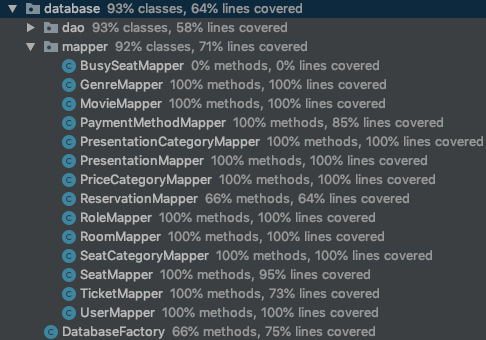
\includegraphics[scale=0.6]{img/testCoverage.png}
		\captionsetup{format=hang}
		\centering\caption[Testabdeckung]{\label{fig:TestCoverage} Übersicht der Testabdeckung}
	\end{figure}
	Die Testabdeckung ist häufig ein faktisches Kriterium für die Qualität des Codes bei Abnahme des Projekts. Beim Erreichen einer bestimmten Prozentzahl fällt allerdings auf, dass diese beim Schreiben der Tests nicht linear steigt. Das liegt daran, dass viele Klassen, die explizit getestet werden, Methoden anderer Klassen wie beispielsweise Superklassen oder Helper-Klassen nutzen. Somit werden diese direkt auch getestet. Andere Klassen wiederum verwenden genau die gleiche Superklasse (oder Helper-Klasse...), die bereits zuvor fremdgetestet wurde. Es sind also weniger Zeilen Code, die für die Testabdeckung zählen, obwohl ähnlich viele Zeilen durchlaufen werden. Daher ist es in der Regel der Fall, dass bei den ersten Tests die Testabdeckung stark wächst, dann jedoch immer langsamer.
	
	\section[Verknüpfung Back- und Frontend]{Verknüpfung Back- und Frontend {\hfill \normalsize tba}}
	REST
	
	\section[Ausblick]{Ausblick {\hfill \normalsize Milena Zahn}}
	%\subsection{Lessons Learned} 
	Die Bereiche, an denen gearbeitet wurde, waren vielfältig. Zuerst waren alle an der Analyse sowie der Erarbeitung des Entwurfs beteiligt. Dann musste sich das Team erarbeiten, wie ein solches Projekt umgesetzt werden kann. Die Programmierung des Backends war für einige der Teammitglieder komplett neu, aber da das Team sehr unterschiedliche Fähigkeiten besitzt, war dies in der geplanten Projektzeit möglich. Auch die Erstellung des Frontends war eine interessante Erfahrung. Die Verbindung von diesem mit dem Backend war für die meisten von uns eine weitere Herausforderung, da in diesem Bereich noch wenige Erfahrungen gemacht wurden. 
	Neben dem technischen Wissen haben die Teammitglieder auch einige weitere Kompetenzen in dem Projekt erworben. Eine davon ist, dass es sehr wichtig ist, andere Projekte, an denen die Teammitglieder außerhalb des Moduls arbeiten müssen, bei dem Projektplans zu berücksichtigen. Obwohl dies sehr schwierig ist, kann dies helfen, den Projektplan genauer und realistischer zu erstellen. Es ist sehr wichtig, für jede Aufgabe genügend Zeit einzuplanen, um unerwartete Herausforderungen zu bewältigen. Die selbständige Erarbeitung von Vorgehensweisen und Lösungskonzepte ist eine weitere in diesem Projekt erworbene Kompetenz.
	Eine weitere Hürde war die Gruppengröße von acht Personen. Es ist schwierig das Potenzial der Gruppe voll ausschöpfen, weil die Arbeit innerhalb der Gruppe gut organisiert werden muss.  Um eine übermäßige Koordination der Mitglieder und lange Kommunikationswege zu vermeiden, haben wir die Gruppe in Untergruppen mit verschiedenen Aufgabenbereichen aufgeteilt. Somit konnte eine schnelle Entscheidungsfindung und kurzfristige Absprachen garantiert werden. Insgesamt wurden in der engen Projektzeit viele unterschiedliche Kompetenzen erworben und vor allem die theoretischen Inhalte der Vorlesung Systemanalyse angewandt.
	